\chapter{Two fission modes in 178Pt}\label{chap:178Pt}

\maketitle

Fission is most well-studied in the region of the actinides (Z=90 to Z=103), as many naturally-occurring isotopes in this region are fissile. Within this region, there is a characteristic tendency for fission fragment yields to be asymmetric (that is, one light fragment and one heavy fragment), with the heavy peak centered around $A\approx140$. This has been understood as a manifestation of nuclear shell structure in the prefragments: doubly-magic $^{132}$Sn drives the nucleus towards scission, and once the neck nucleons are divided up between the two fragments, we end up with the heavy fragment A=140 peak. As one moves to the lower-Z actinides, however, this tendency becomes less and less pronounced as yields tend to become more symmetric. Below thorium, it was generally believed (though mostly not tested) that yields would continue to be symmetric as there was no doubly-magic nucleus candidate that could reasonably be expected to drive the system toward asymmetry as there is with actinides.

However, it was reported in a paper published in 2010 \cite{Andreyev2010} that neutron-deficient $^{180}$Tl undergoes beta-delayed fission, leading to intermediate state $^{180}$Hg which then decays into two fragments of unequal mass. This finding triggered a flurry of theoretical papers hoping to describe this new and unexpected phenomenon. A follow-up study using $^{180}$Tl \cite{Liberati2013} around the same time established this as a region of asymmetric fission, and not just a one-time occurence. Since then, other nuclei in the region have been studied, for instance, using Coulex-induced fission reactions and compound nucleus (prompt?) fusion-fission reactions, and the finding is the same. Furthermore, experiments done at different excitation energies have shown that, unlike the case of actinides where shell structure and fragment asymmetry is ``washed out'' at high excitation energies, mass asymmetric mass distributions are a persistent feature of this mass distribution for various excitation energies. (A lot of good citations for this section can come from section 4.1.1 of \cite{Andreyev2018})

Predicted fission barrier heights in this region are relatively-low (of the order of ~12 MeV), making them suitable for study using low-energy techniques such as $\beta$-delayed fission (maybe \cite{Andreyev2013} and the work at ISOLDE at CERN?) or Coulex-induced fission (maybe \cite{Martin2015} and the SOFIA (Studies On FIssion with Aladin) experiment/project/campaign). On the other hand, it has been found that compound nuclei formed in this region from particle-induced reactions tend to have hig excitation energies, even for beam energies near the Coulomb barrier. This combination makes the region particularly well-suited for studies involving a variety of excitation. This region was being studied for fission at different excitation energies, whn it was discovered - quite by accident - that it fissioned asymmetrically.

A follow-up experiment was performed in 20?? \cite{our-Pt-paper} investigating spontaneous fission of $^{178}Pt$, which differs from $^{180}$Hg by 2 protons. This system was studied at various excitation energies and found to fission pretty consistently with a bimodal pattern. Of the nuclei which underwent spontaneous fission, roughly 1/3 were found to fission symmetrically while the other 2/3 fissioned asymmetrically with a light-to-heavy mass ratio of approximately 80/98 (Is that the correct ratio?). Furthermore, it was observed that symmetric fragments tended to have higher kinetic energies than non-symmetric fragments. 

\begin{figure}
	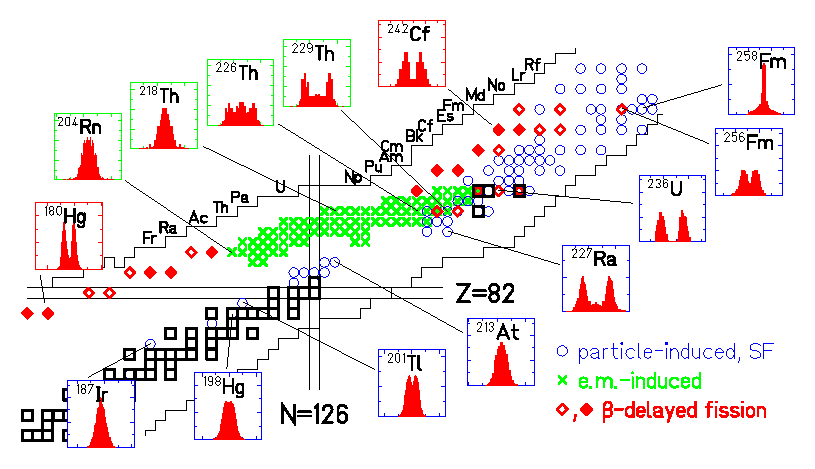
\includegraphics[width=0.9\linewidth]{./TeX_files/with180Hg}
	\caption[Short]{Fragment yields for several nuclei ranging from actinides, where primary fission yields tend to be asymmetric, down to near-thorium, where yields become more symmetric except in the region near neutron deficient $^{180}$Hg. Figure from \cite{Andreyev2010}. [NOTE: There's an updated version in \cite{Andreyev2018}]}
	\label{fig:with180hg}
\end{figure}

Elongation tends to minimize the Coulomb repulsion between fragments

Why is there a region of symmetric fission below thorium?